\definecolor{yellow}{rgb}{1.0, 1.0, 0.45} % 255/255/115
\definecolor{dkyellow}{rgb}{0.9, 0.9, 0.0} % % 230/230/0

\definecolor{ltorange}{rgb}{1.0, 0.74, 0.41} % 255/188/105
\definecolor{orange}{rgb}{0.96, 0.50, 0.0} % 246/127/0

\definecolor{ltred}{rgb}{1.0, 0.25, 0.25} % 255/64/64
\definecolor{red}{rgb}{0.79, 0.00, 0.01} % 201/0/3

\definecolor{ltpurple}{rgb}{0.81, 0.57, 1.00} % 206/145/255
\definecolor{purple}{rgb}{0.38, 0.00, 0.68} % 97/1/175

\definecolor{ltblue}{rgb}{0.2, 0.73, 1.0} % 51/187/255
\definecolor{blue}{rgb}{0.12, 0.43, 0.59} % 30/110/150

\definecolor{ltltgreen}{rgb}{0.7, 1.00, 0.7} % 96/204/14
\definecolor{ltgreen}{rgb}{0.37, 0.80, 0.05} % 96/204/14
\definecolor{green}{rgb}{0.23, 0.49, 0.03} % 59/125/8
  
\definecolor{dkslate}{rgb}{0.18, 0.21, 0.28} % 47/53/72
\definecolor{mdslate}{rgb}{0.45, 0.50, 0.68} % 114/127/173
\definecolor{ltslate}{rgb}{0.85, 0.88, 0.95} % 216/225/229

\tikzstyle{phase} = [rectangle, 
                      draw=dkyellow!80!black,
                      top color=yellow,
                      bottom color=dkyellow]
\tikzstyle{cig} = [rectangle, 
                      rounded corners=0.5em,
                      draw=orange!80!black,
                      top color=ltorange!50!white,
                      bottom color=orange]
\tikzstyle{open} = [rectangle, 
                      rounded corners=0.5em,
                      draw=green!80!black,
                      top color=ltgreen!20!white,
                      bottom color=green]
\tikzstyle{free} = [rectangle, 
                      rounded corners=0.5em,
                      draw=blue!80!black,
                      top color=ltblue!20!white,
                      bottom color=blue]
\tikzstyle{commercial} = [rectangle, 
                      rounded corners=0.5em,
                      draw=ltred!80!black,
                      top color=ltred!20!white,
                      bottom color=red!70!white!100]
\tikzstyle{available} = [thick, color=black]
\tikzstyle{planned} = [thick, dashed, color=mdslate]


\begin{center}
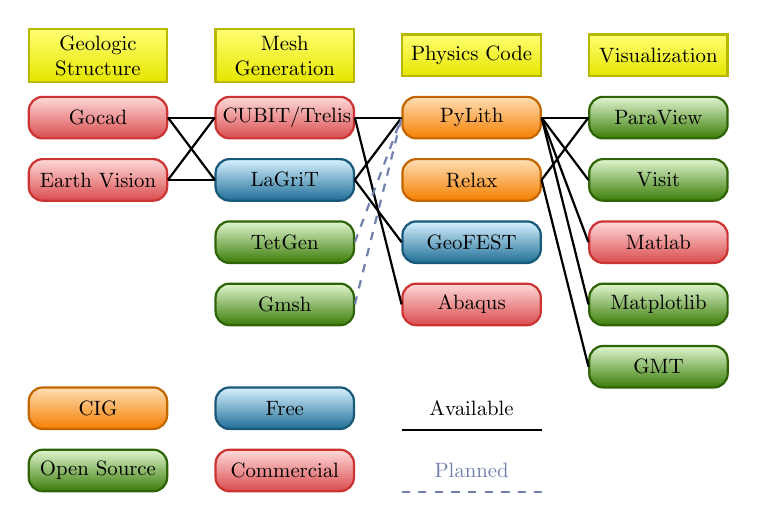
\begin{tikzpicture}[scale=0.75, transform shape,
  node distance=3.0em,
  text width=6em, text centered, minimum height=2em, thick]

  % Phases
  \node (structure) [phase] {Geologic Structure};
  \node (meshing) [phase, right of=structure, xshift=6em] {Mesh Generation};
  \node (physics) [phase, right of=meshing, xshift=6em] {Physics Code};
  \node (viz) [phase, right of=physics, xshift=6em] {Visualization};

  % Geologic structure
  \node (gocad) [commercial, below of=structure] {Gocad};
  \node (earthviz) [commercial, below of=gocad] {Earth Vision};

  % Mesh generation
  \node (cubit) [commercial, below of=meshing] {CUBIT/Trelis};
  \node (lagrit) [free, below of=cubit] {LaGriT};
  \node (tetgen) [open, below of=lagrit] {TetGen};
  \node (gmsh) [open, below of=tetgen] {Gmsh};

  % Physics code
  \node (pylith) [cig, below of=physics] {PyLith};
  \node (relax) [cig, below of=pylith] {Relax};
  \node (geofest) [free, below of=relax] {GeoFEST};
  \node (abaqus) [commercial, below of=geofest] {Abaqus};

  % Visualization
  \node (paraview) [open, below of=viz] {ParaView};
  \node (visit) [open, below of=paraview] {Visit};
  \node (matlab) [commercial, below of=visit] {Matlab};
  \node (matplotlib) [open, below of=matlab] {Matplotlib};
  \node (gmt) [open, below of=matplotlib] {GMT};

  % Paths
  \path (gocad.east) edge[available] (cubit.west);
  \path (gocad.east) edge[available] (lagrit.west);
  \path (earthviz.east) edge[available] (cubit.west);
  \path (earthviz.east) edge[available] (lagrit.west);

  \path (cubit.east) edge[available] (pylith.west);
  \path (cubit.east) edge[available] (abaqus.west);
  \path (lagrit.east) edge[available] (pylith.west);
  \path (lagrit.east) edge[available] (geofest.west);
  \path (tetgen.east) edge[planned] (pylith.west);
  \path (gmsh.east) edge[planned] (pylith.west);

  \path (pylith.east) edge[available] (paraview.west);
  \path (pylith.east) edge[available] (visit.west);
  \path (pylith.east) edge[available] (matlab.west);
  \path (pylith.east) edge[available] (matplotlib.west);
  \path (relax.east) edge[available] (paraview.west);
  \path (relax.east) edge[available] (gmt.west);

  % Legend
  \node (cig) [cig, below of=earthviz, yshift=-8em] {CIG};
  \node (open) [open, below of=cig] {Open Source};
  \node (free) [free, right of=cig, xshift=6em] {Free};
  \node (commercial) [commercial, below of=free] {Commercial};

  \node (available) [available, right of=free, xshift=6em] {Available};
  \path (available.south west) edge[available] (available.south east);

  \node (planned) [planned, below of=available] {Planned};
  \path (planned.south west) edge[planned] (planned.south east);


\end{tikzpicture}
\end{center}
\vfill
